\documentclass[10pt,a4paper]{report}
\usepackage[utf8]{inputenc}
\usepackage{amsmath}
\usepackage{amsfonts}
\usepackage{hyperref}
\usepackage{amssymb}
\usepackage{tikz-cd}
\usepackage {tikz}
\usepackage{lipsum}
\usetikzlibrary{arrows, positioning, automata}
\usetikzlibrary {positioning}
%\usepackage {xcolor}
\definecolor {processblue}{cmyk}{0.96,0,0,0}

\author{Alexandre Sallinen, Salim Najib}
\begin{document}
\newcommand{\code}[1]{\texttt{#1}}

\section*{\centering{Rapport: Rigel étape 12}}

\section*{Graphes et ensembles}

Le paquetage \code{math} est enrichi de \code{sets}, comptant nombre de définitions d'ensembles avec des opérations telles que la partition pour \code{PartitionSet} et l'équation dans \code{Equation}. Ceci facilite l'écriture de \code{graphs}, qui comprend, entre autres, la définition d'un arbre générique \code{Tree<T>}. Ces deux nouveaux sous-paquetages sont utiles dans l'implémentation de nombre des ajouts décrits ci-dessous.

\section*{Ajouts principaux}

\subsection*{Barre de recherche}

La barre de recherche permet à l'utilisateur de chercher un objet céleste via son nom. A chaque lettre tapée, l'utilisateur voit une liste des objets célestes commençant par la même séquence de lettres que celles entrées. Cliquer sur un nom centre la projection sur l'objet choisi.

L'implémentation de cette barre de recherche passe par \linebreak\code{...gui.searchtool.SearchTextField}, classe abstraite qui représente une barre de recherche générale capable de fournir un objet (celui séléctionné au terme de la recherche). Le \code{Searcher} constitue une implémentation de cette classe qui se spécialise dans les objets célestes. Pour effectuer une recherche rapide, les noms des objets célestes sont entrés dans un \code{Tree<Character>} où chaque mot est décomposé par lettres, et appartiennent à une même branche les mots qui ont une séquence de lettres identique jusqu'à un certain indice.

\subsection*{Parallélisme}

Afin d'améliorer la performance du programme et diminuer les saccades, \linebreak\code{...parallelism.ThreadManager} génère un arbre de tâches à effectuer et assigne les tâches à une réserve de threads.

L'annotation \code{Requires} indique quels \textit{stages} devront être complétés avant que ne soit exécuté celui au-dessus duquel elle se situe. Les tâches sont alors organisées dans un graphe, plus précisément une forêt. Dans chaque arbre, les feuilles constituent les premières tâches à effectuer. Les tâches plus proches de la racine nécessitent la complétion des précédentes avant d'être exécutées.

\begin{figure}
\centering
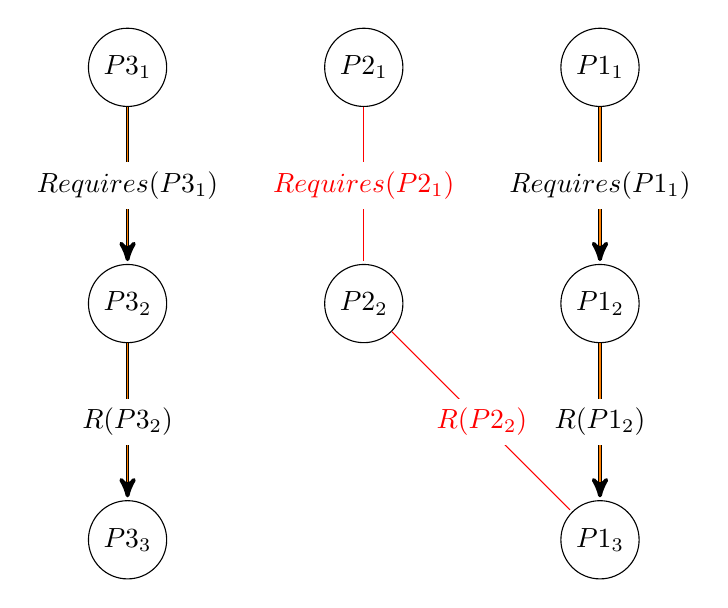
\begin{tikzpicture}[>=stealth',shorten >=1pt,node distance=3cm,on grid,initial/.style={}]

state/.style ={ circle ,top color =white , bottom color = processblue!20 ,
draw,processblue , text=blue , minimum width =1 cm}]

    \node[state] (P1) {$P1_1$};
    \node[state] (P2) [left  =of P1]{$P2_1$};
    \node[state] (P3) [left  =of P2]{$P3_1$};

    \node[state] (P12) [below =of P1] {$P1_2$};
    \node[state] (P22) [below =of P2] {$P2_2$};
    \node[state] (P13) [below =of P12] {$P1_3$};
    \node[state] (P32) [left =of P22] {$P3_2$};
    \node[state] (P33) [below =of P32] {$P3_3$};

    \tikzset{mystyle/.style={->,double=orange}}
    \tikzset{every node/.style={fill=white}}
    \path (P1)  edge  [mystyle] node {$Requires(P1_1)$} (P12);
    \path (P2)  edge  [red] node {$Requires(P2_1)$} (P22);
    \path (P3)  edge [mystyle] node {$Requires(P3_1)$} (P32);
    \path (P12) edge [mystyle] node {$R(P1_2)$} (P13);
    \path (P22) edge [red] node {$R(P2_2)$} (P13);
    \path (P32) edge [mystyle] node {$R(P3_2)$} (P33);

	

\end{tikzpicture}
\caption{Un graphe possible des taches}
\end{figure}

Chaque $PN_i$ représente un \textit{processus} qui sera exécuté par le gestionnaire. En rouge : une branche qui sera exécuté par les mêmes threads en parallèle de ses branches adjacentes mais qui attendra la complétion de la branche des $P1_i$ pour continuer en $P1_3$. 

\section*{Ajouts secondaires}

\subsection*{Prédiction d'orbite}

La prédiction d'orbite permet de connaître, avec clic droit sur des planètes, la Lune ou le Soleil, leur trajectoire à venir. Ces futures positions sont modélisées par des points dont l'espacement est modifiable.

Ces orbites font usage de \code{graphs} en héritant des \code{Cycles}, des graphes cycliques. Ainsi, l'orbite n'est qu'un \code{Cycle} de \linebreak\code{Supplier<CelestialObjectModel>} pour limiter le calcul, et ce sont les paramètres d'espacement qui permettent de récupérer des positions avec une certaine périodicité. L'espacement entre les représentants de l'orbite est une visualisation de la vitesse de l'objet.

\subsection*{Gestion des paramètres d'interface graphique}

Le bouton labellisé d'un rouage à coté de la barre de recherche ouvre un panneau de réglages graphiques : un mode \textit{cinématique} cachant l'interface utilisateur pour ne laisser que le ciel, une touche permettant d'activer ou de désactiver
le \hyperref[sec:info]{paneau d'information}, un mode plein écran, et un bouton restreignant la vue au ciel réellement visible (interdiction d'observer sous la barre des $5^{\circ}$ d'hauteur). Ensuite, deux paramètres de sensibilités de souris sont proposés. Pour finir, de nombreux paramètres graphiques gérant la couleur, les éléments à dessiner et l'espacement de la grille horizontale sont présentés.

Le plein écran joue sur un simple paramètre du BorderPane (\code{setFullScreen}); le masquage du panneau de droite, la restriction d'altitude et le mode cinématique sont gérés par des propriétés booléennes misent en place dans le \code {Main} et \linebreak\code{SkyCanvasManager}.
Les sliders agissent quant à eux sur des valeurs définies dans \code{SkyCanvasManager}. Enfin les paramètres de couleurs et d'affichages sont modélisés de manière similaire, le \code{SkyCanvasPainter} ayant la capacité de changer la couleur de certains de ces éléments et les \code{Checkboxes} activant ou désactivant des parties du ciel, s'aidant de l'enum \code{...gui.DrawableObjects}.


\subsection*{Informations sur les corps célestes}

\label{sec:info}
La barre de droite du BorderPane affiche, lorsqu'un corps céleste est séléctionné via clic droit, des propriétés générales telles que ses coordonnées équatoriales, ainsi que des infos spécifiques à son type, par exemple : température et hipparcos pour les étoiles, ainsi que les étoiles dans la même constellation. Des sliders s'afficheront également pour modifier l'affichage de prédiction d'orbite des constituants du système solaire.

Pour trouver les étoiles dans une même constellation, la méthode \linebreak \code{StarCatalogue.constellationOfStar(Star)} fournit un getter pour la map \code{Map<Star, AbstractMathSet<Star>> constellationsMap} qui relie, à chaque étoile, l'ensemble des étoiles dans la même constellation qu'elle. La \code{Map} permet un accès en $\mathcal{O}(1)$.

\subsection*{Mouvements de souris et rotation du ciel}

Enfin, glisser la souris avec clic gauche enfoncé modifie le centre de projection, et la glisser avec roulette enfoncée modifie la rotation du ciel. 

\subsection*{ }

Plus d'informations sur les contrôles et fonctionnalités sont disponibles en cliquant sur le bouton d'aide, à droite de celui ouvrant les paramètres.

\subsection*{ }

Vous remerciant pour un projet -et un cours!- passionnants malgré les contraintes exceptionnelles, 

\subsection*{ }

\mbox{}\hfill Alexandre Sallinen et Salim Najib.

\end{document}